
\begin{figure}

	\begin{subfigure}[t]{0.48\textwidth}
		\center
		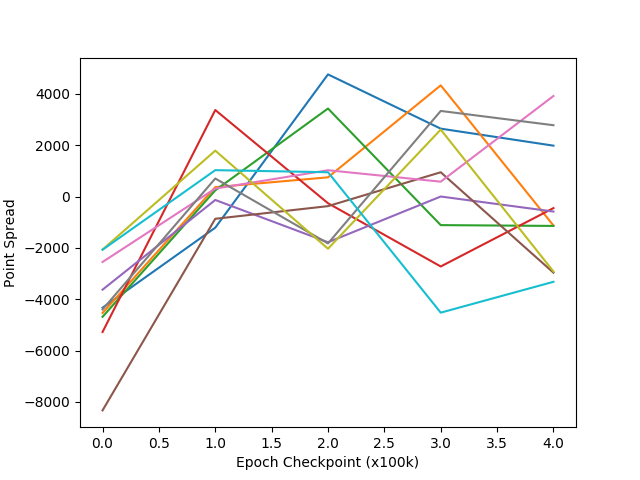
\includegraphics[width=\textwidth]{images/findings/experiments/regularization/tourny/reg_050-kyttuhat-strict-500k.png}
		\caption{$r = 0.50$}
	\end{subfigure}
	~
	\begin{subfigure}[t]{0.48\textwidth}
		\center
		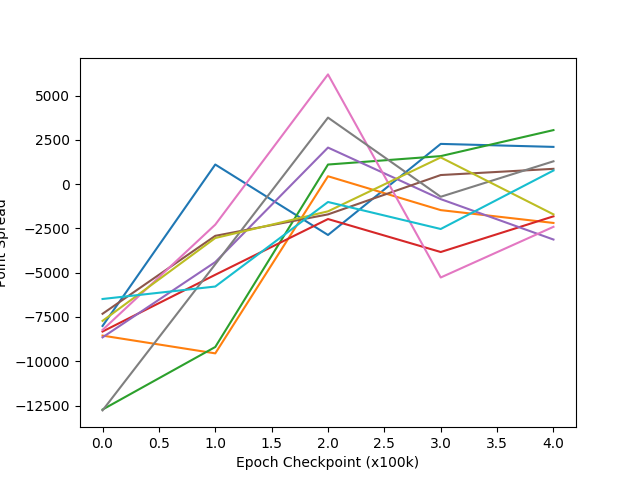
\includegraphics[width=\textwidth]{images/findings/experiments/regularization/tourny/reg_060-kyttuhat-strict-500k.png}
		\caption{$r = 0.60$}
	\end{subfigure}

	\begin{subfigure}[t]{0.48\textwidth}
		\center
		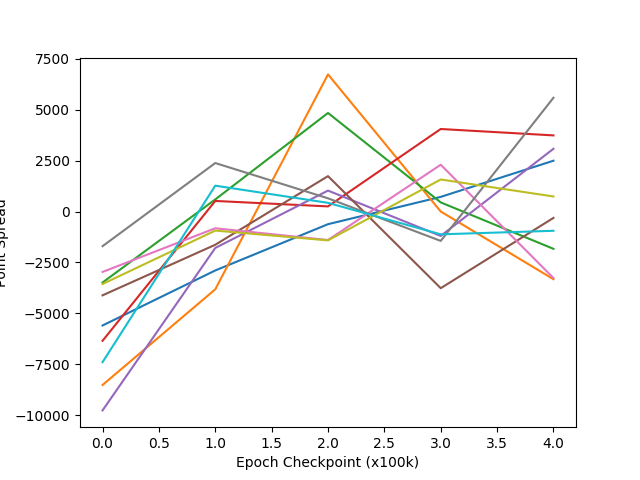
\includegraphics[width=\textwidth]{images/findings/experiments/regularization/tourny/reg_070-kyttuhat-strict-500k.png}
		\caption{$r = 0.70$}
	\end{subfigure}
	~
	\begin{subfigure}[t]{0.48\textwidth}
		\center
		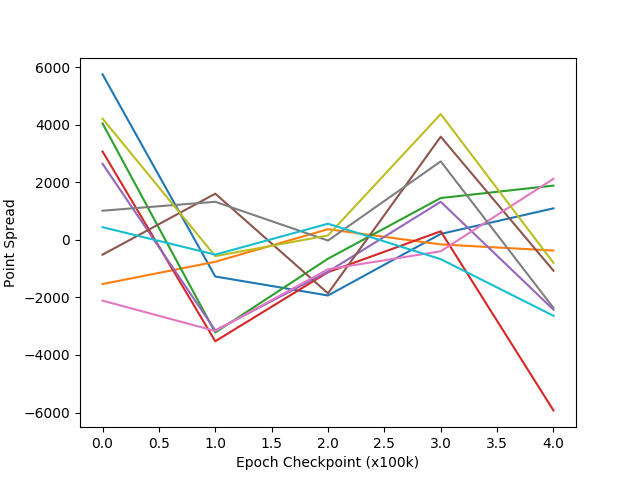
\includegraphics[width=\textwidth]{images/findings/experiments/regularization/tourny/reg_080-kyttuhat-strict-500k.png}
		\caption{$r = 0.80$}
	\end{subfigure}

\caption{
	Point spreads of self-tournaments for 10,000 games
	carried out between agents trained using
	the regulation method mentioned in Section~\ref{sec:findings-r2} after being
	trained for 500,000 games.
	Each tournament plot in n this figure is referenced by the regularization
	rate $r$ in use during training.
}
\label{fig:reg-tournies}
\end{figure}
